\hypertarget{ClasseLeitorExibidor_8cpp}{}\section{Referência ao ficheiro src/\+Classe\+Leitor\+Exibidor.cpp}
\label{ClasseLeitorExibidor_8cpp}\index{src/\+Classe\+Leitor\+Exibidor.\+cpp@{src/\+Classe\+Leitor\+Exibidor.\+cpp}}


Classe que irá realizar a leitura do bytecode e salvar as informações do class file.  


{\ttfamily \#include \char`\"{}Classe\+Leitor\+Exibidor.\+h\char`\"{}}\newline
Diagrama de dependências de inclusão para Classe\+Leitor\+Exibidor.\+cpp\+:
\nopagebreak
\begin{figure}[H]
\begin{center}
\leavevmode
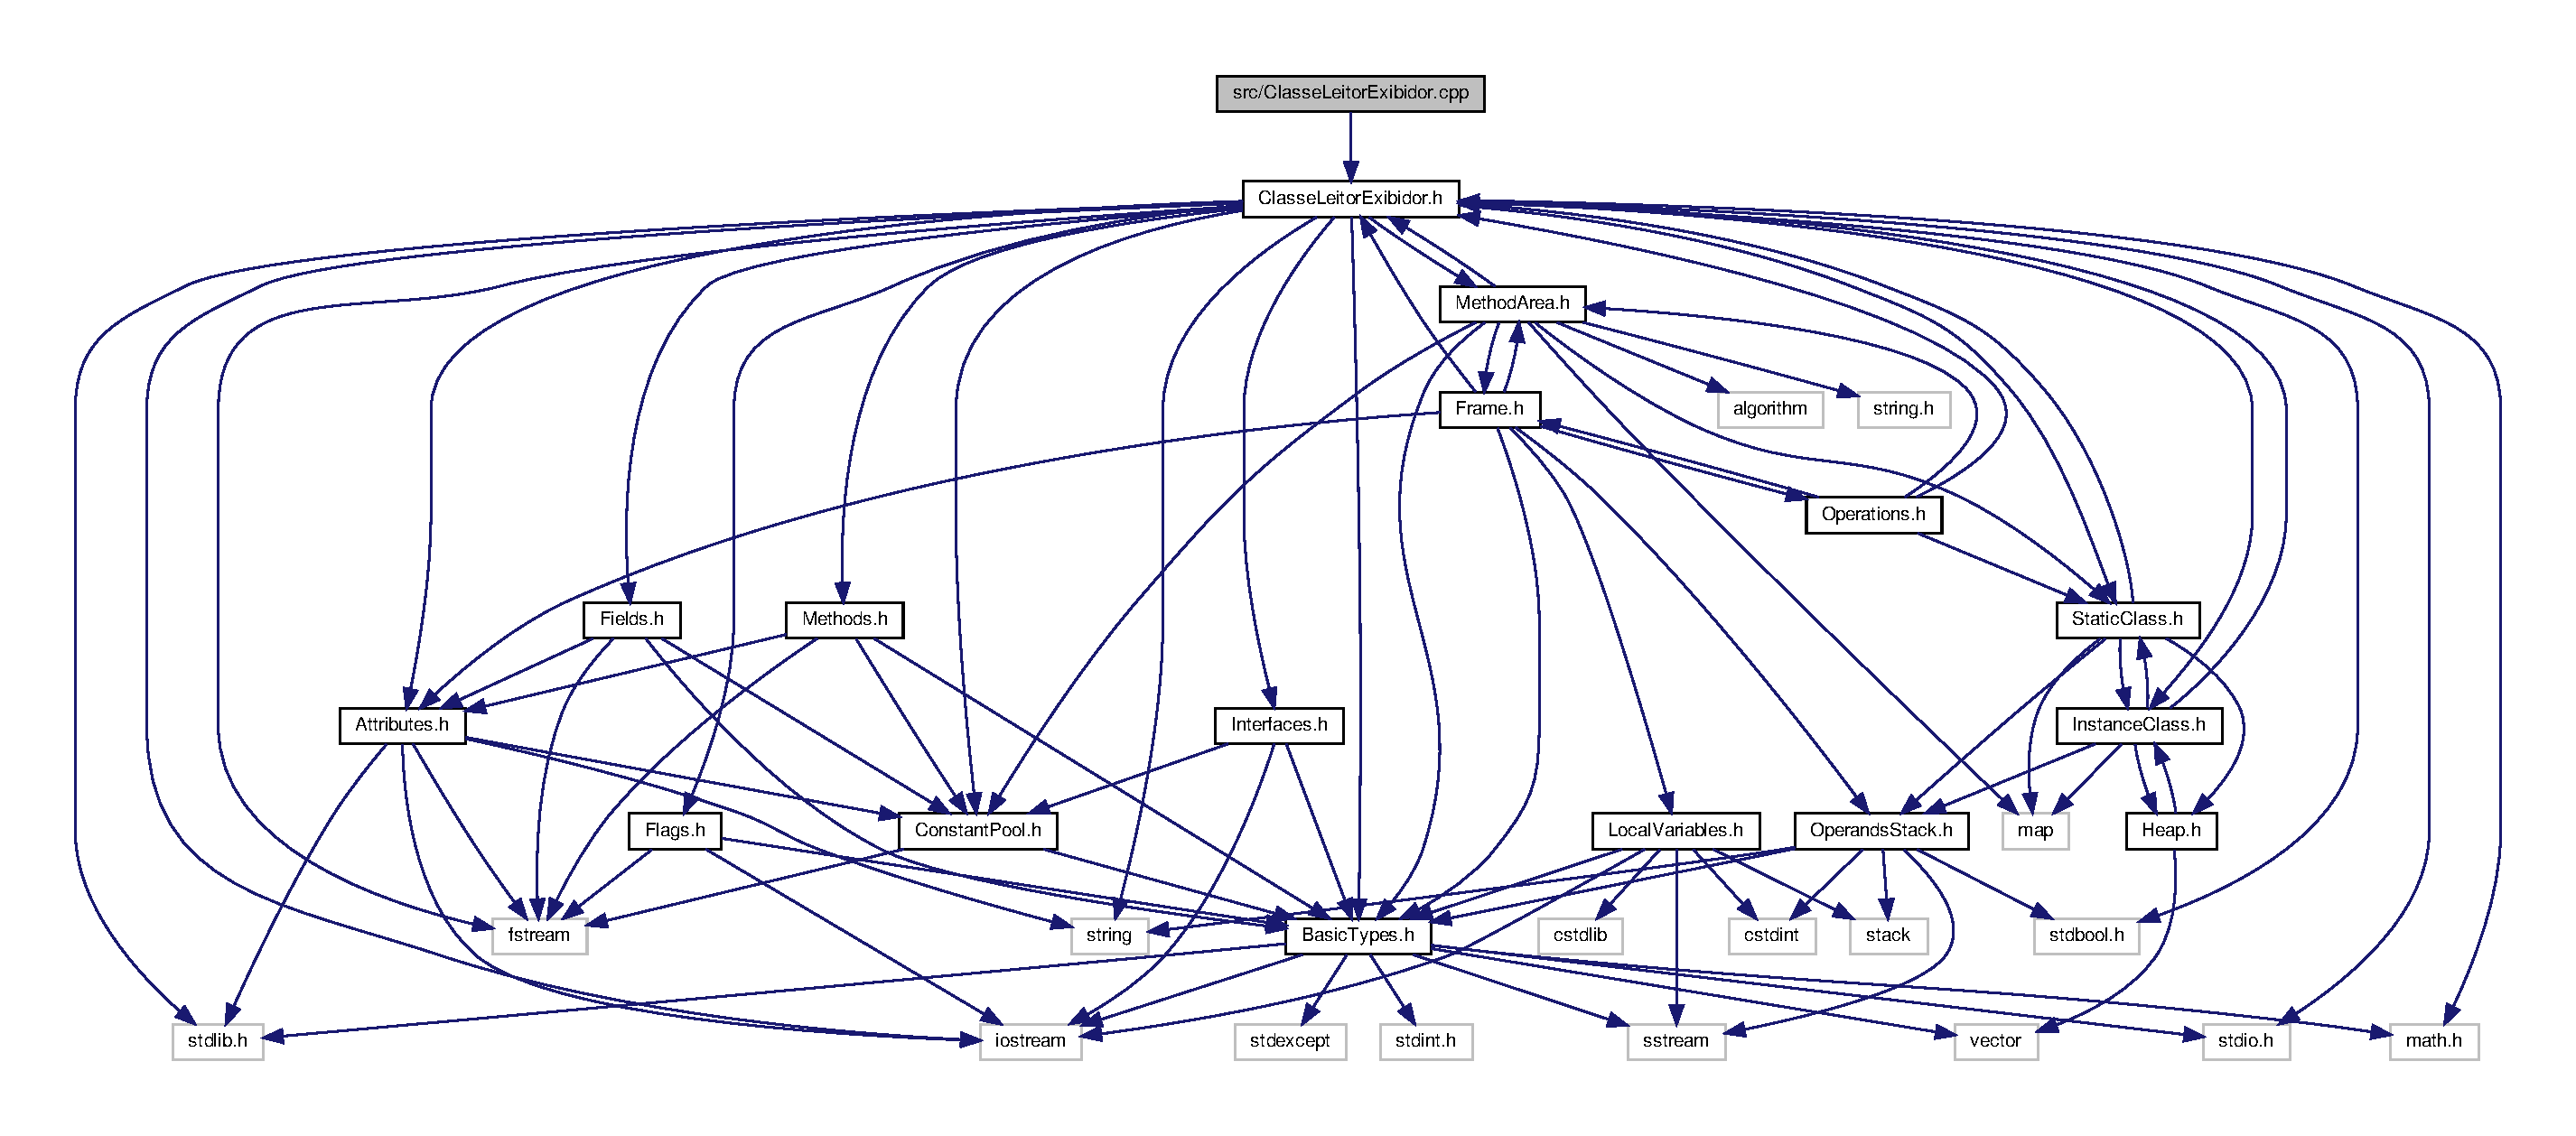
\includegraphics[width=350pt]{ClasseLeitorExibidor_8cpp__incl}
\end{center}
\end{figure}


\subsection{Descrição detalhada}
Classe que irá realizar a leitura do bytecode e salvar as informações do class file. 

